\clearpage
\newpage % 开始新的一页
    \thispagestyle{empty} % 移除本页的页眉和页脚[8,9](@ref)
    \newgeometry{margin=0pt} % 临时将本页的页边距全部设置为0[1](@ref)
    \noindent % 防止缩进
    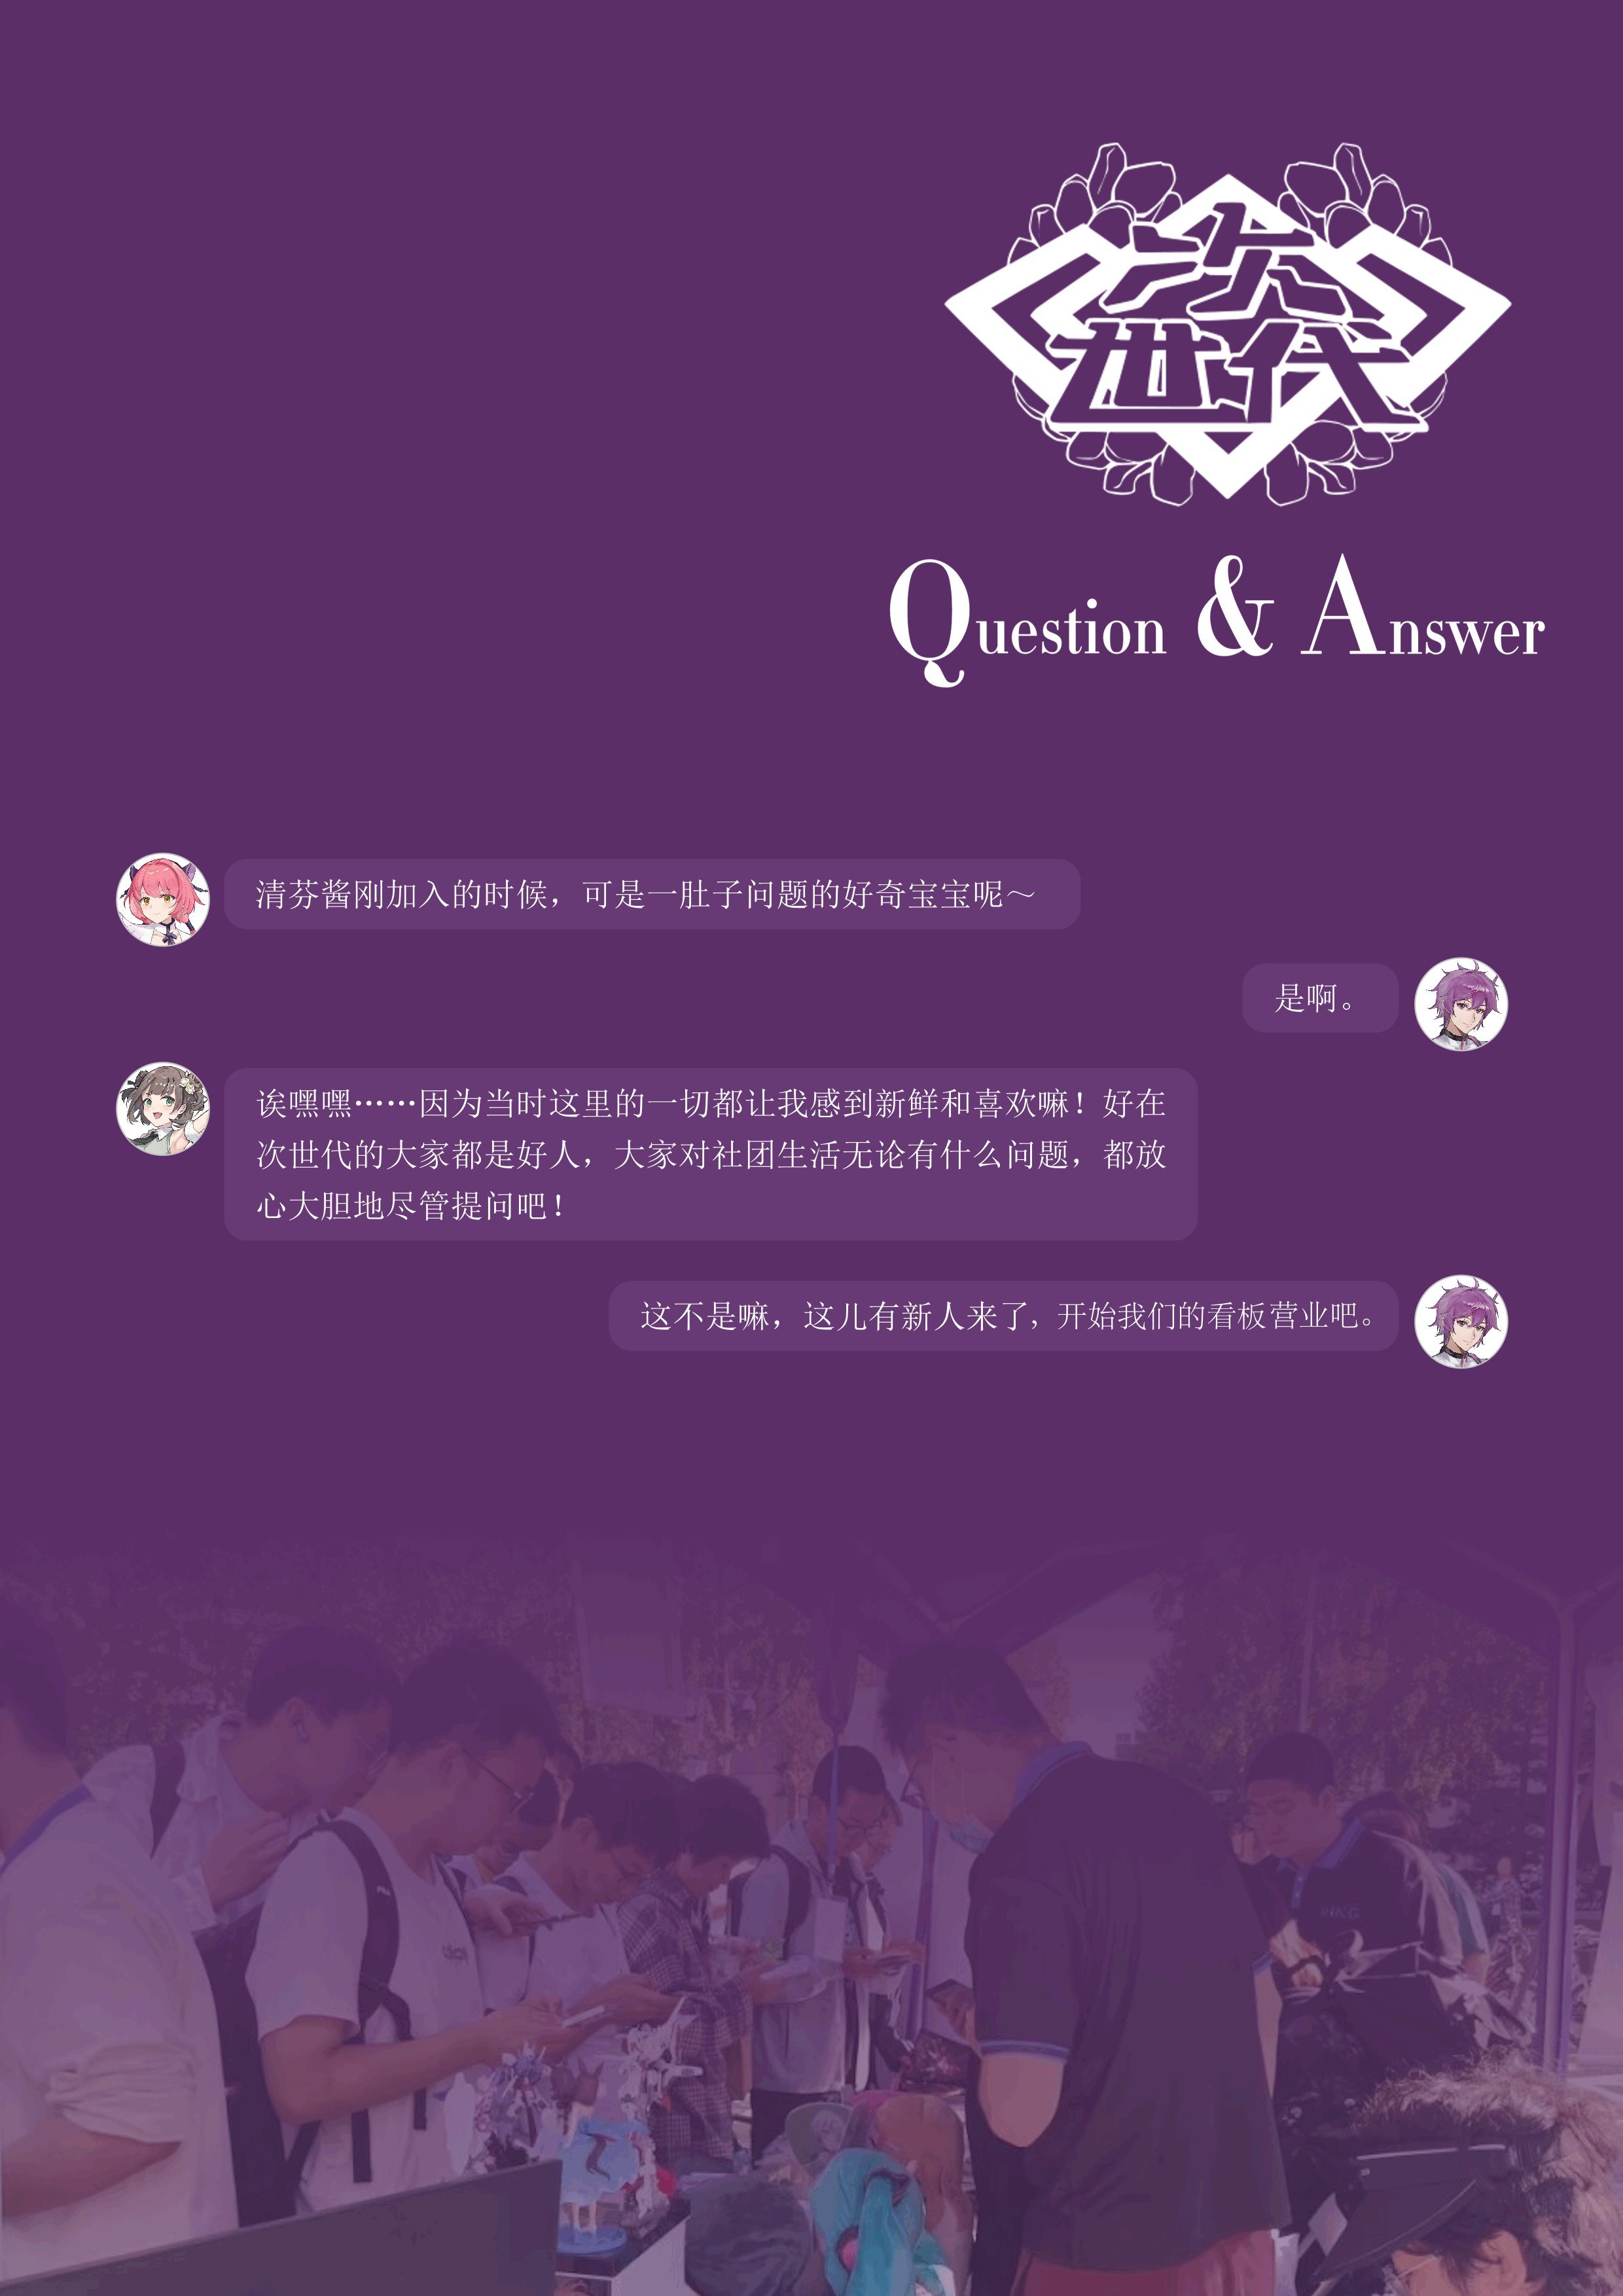
\includegraphics[width=0.9999\paperwidth, height=0.9999\paperheight]{ch3.jpg} % 插入图片,使其尺寸与纸张大小一致并保持宽高比[1](@ref)
    \restoregeometry % 恢复原来的页边距设置
\normalsize
\vspace{2em}
\par
\chatbubble[left]{yui.jpg}{阿梓喵呆suki}{
 呃……我好像还是不知道如何加入次世代……
}{default}

\chatbubble[right]{zijing.jpg}{紫荆}{
浏览器访问thujsd.club 或者扫描手册封底的二维码,一步一步按照提示来就可以啦。具体来说,网站会引导你通过清华账号注册成为社员,然后加入次世代QQ主群,你就是次世代社员了。没有网站注册过是无法加入主群的,所以直接邀请朋友进群是不行的,要记住哦。
}{zi}

\chatbubble[left]{qiya.jpg}{奇犽}{
 除了刚刚的介绍,次世代还有哪些活动呀?
}{default}

\chatbubble[right]{taozi.jpg}{桃子没有在摸鱼}{
 最主要就是各分部自发组织的活动啦,如绘画部的茶绘、动研部的新番研讨会、
 地下live部的应援例会、东方部的东方例会、Lolita部的茶话会、各个二游部的集体赌博
 (给赌博来个划掉的效果)抽卡等等。未来无论是社团还是分部还会有更多的活动需要由你们来建设,
 快来和桃子一起搞波大的吧~
}{tao}

\chatbubble[left]{yagami.jpg}{专业代签名送苹果​}{
你们说的这个ID/cn是怎么一回事?
}{default}

\chatbubble[right]{taozi.jpg}{桃子没有在摸鱼}{
为了保证充分的自由空间\sout{防社死},我们的文化是匿名玩耍~ID/cn (coser name)其实就是你的网名/昵称,在次世代你可以使用它,在不暴露你的院系和姓名的情况下尽情开心。不过这可不能成为你不遵守发言规范和社交基本原则的理由哟~
}{tao}

\chatbubble[left]{guitarhero.jpg}{吉他英雄}{
  加入动漫社……是不是意味着要参加好多好多线下活动?要自我介绍?要上舞台?
  这个绝对做做做做做做做做不到!
}{default}

% 右侧聊天(用户B)
\chatbubble[right]{qingfen.jpg}{清芬哒哟}{
 绝对没这回事!我们所有的活动都是自愿参加的!当然,我们欢
 迎每一位社员的热情。但是就算只是来咖啡厅买一杯特调,来社庆做
 一枚静静的观众,或在群聊里默
 默收集好看的图片也都没问题!我们的宗旨就是玩得开心~
}{qing}
\newpage 
\chatbubble[left]{zijing.jpg}{紫荆(四肢驯服中)}{
 不会跳舞可以加入宅舞部吗。?
}{zi}

\chatbubble[right]{taozi.jpg}{桃子没有在摸鱼}{
 当然可以!宅舞部很多都是0基础的朋友噢~只要热爱就可以加入,
 大家会一起学舞一起练习的(抱大腿)喜欢您来!
}{tao}

\chatbubble[left]{mortis.jpg}{若叶睦(Mortis 版)}{
 想加入创作部门,但无论乐队还是绘画、cosplay,全~都不会!
}{default}

\chatbubble[right]{qingfen.jpg}{清芬哒哟}{
 没关系,大部分人都和你一样!正是因此,几乎每个创作部门招新时都会强调:
 我们部门从不拒绝零基础选手,我们有热心太太组成的资深团队,帮助每个虚心求教的萌新快速入门!
}{qing}

\chatbubble[left]{konami.jpg}{(该用户未填写昵称)}{
 我的品味小众又独特,该如何在次世代找到同好呢?
}{default}

\chatbubble[right]{taozi.jpg}{桃子没有在摸鱼}{
 次世代最不缺的就是小众作品爱好者(此处应有一张部门全表),只要多水群,找不到同好比找到同好还难呢!
 此外,我们秉承“三人成部”传统,只要再有两位同好,就可以申请成立一个新部门~如果你有感兴趣的领域
 还没有部门,欢迎来找我们哦!
}{tao}

\chatbubble[left]{shishangyou.jpg}{冻鳗领域大神}{
 如何向大家推荐我喜欢的作品?
}{default}

\chatbubble[right]{zijing.jpg}{紫荆}{
 有很多种方式。次世代动画研究会(简称动研部)会定期举办新番研讨会,这是安利作品、分享见解的最好机会。
 此外,次世代放映组每周都会组织放映会,现在加入放映部,完成登记和教室预约后,就可以申请放映自己喜欢的作品了。
}{zi}

\chatbubble[left]{tamako.jpg}{兔子山商店街欢迎您来}{
 我也想为次世代的活动出一份力~我该如何来帮忙打工?
}{default}

\chatbubble[right]{qingfen.jpg}{清芬哒哟}{
 次世代组织部欢迎你的加入!组织部每周都会举办例会,分配下一周的工作任务。
 值得一提的是,所有任务都是自愿接受的,例会只来旁听也完全没问题~
 在主题咖啡厅、社庆等大型活动前,组织部群里还会发布志愿者招募公告,填写问卷后就可以成为帕鲁啦!
 大型活动的帕鲁可能还会有神秘福利哦!
}{qing}





\chatbubble[left]{haruhi.jpg}{非外星人未来人超能力者勿扰}{
 我要拉我别的学校的朋友一起来玩!
}{default}

\chatbubble[right]{qingfen.jpg}{清芬哒哟}{
呃……如果是来参加活动的话没问题!次世代的各大活动都是向所有人开放的!虽然很抱歉,由于相关规定,次世代主群暂时不接受外校同学进入……不过各个分部如何规定是自由的,有不少分部允许信得过的同学加入~
}{qing}

\chatbubble[left]{rika.jpg}{极东魔术昼寝结社の夏社长}{
 次世代会和其他社团合作举办活动吗?
}{default}

\chatbubble[right]{zijing.jpg}{紫荆}{
 时常会有。最常见合作的是友校的各大动漫社,如北大元火动漫社。此外本校的话,次世代放映部不时会和学生科幻协会合作举办科幻电影放映会;主题咖啡厅也是外社
 联动的常客,荷月玩偶社、学生科幻协会等都曾是我们的联动对象。此外,学生电子音乐协会、学生推理协会
 也曾和我们有过合作。如果有任何想要进行外社联动的想法,欢迎联络组织部。
}{zi}

\chatbubble[left]{wohenhaoqi.jpg}{好奇宝宝}{
 我对次世代的历史很好奇!
}{default}

\chatbubble[right]{zijing.jpg}{紫荆}{
1999年,以电子游戏为主题的次世代文化与娱乐协会成立,不久便向ACGN爱好者的集合体转变。2011年,改名为“次世代动漫社”,初步具备了现在的样貌,并开始举办以社庆为代表的系列活动。11年起有许多老人直到现在都在各大群聊活跃着,可以向他们打听他们的传说。
}{zi}

\chatbubble[left]{shinnku.jpg}{半透明的魔法使}{
加入分部团体但是在部内没有认识的同学怎么办?会不会没有办法融入集体,被大家接纳呢?我想,言语是具有魔法的……如果得到的只是陌生冷漠的言语,我似乎很难继续待在这里……
}{default}

\chatbubble[right]{taozi.jpg}{桃子没有在摸鱼}{
不用担心,次世代的各个分部的前辈们绝大多数都是十分开放友好的,对新人十分欢迎的~毕竟,让一个部门、一个群聊永葆生命,必须要有新鲜血液的加入!部门的介绍,部门活动的指导往往可以通过群文件或者精华消息得知,就算有什么不懂的,以友好的语气大胆发问,热情的群友会帮助你的~就算没有办法融入某个部门,次世代有几百个部门,总有与你“对上电波”的地方存在的!
}{tao}

\chatbubble[left]{kuro.jpg}{夜之国的小猫}{
次世代有许多与动漫似乎无关的部门(例如许多学习相关的部门),这些部门具体会做些什么呢,和次世代的关系又是什么呢?
}{default}

\chatbubble[right]{zijing.jpg}{紫荆}{
这些部门本身的职能可能确实不太“二次元”,但是里面的成员作为次世代社员,很可能(?)都是二次元。次世代为了同好人群而服务,而这些部门能帮助你与群友在有二次元的同好的基础上能在学习生活各方面找到共同话题,说不定能更加简单的成为好友(这就是二次元之间的“羁绊”啊)。同时,这些部门更加贴近学习生活,可能会有更丰富的线下活动组织和具体建议指导,相信一定能让你的大学生活更加丰富多彩。
}{zi}

